\documentclass[twocolumn]{aastex631}

\usepackage{amsmath}
\usepackage{graphicx}
\usepackage{natbib}

\newcommand{\vplanet}{\texttt{VPLanet}}
\newcommand{\vconverge}{\texttt{vconverge}}
\newcommand{\Fxuv}{F_{\mathrm{XUV}}}
\newcommand{\Fcum}{F_{\mathrm{XUV,cum}}}
\newcommand{\Fearth}{F_{\oplus,\mathrm{XUV,cum}}}
\newcommand{\Msun}{M_{\odot}}
\newcommand{\Mearth}{M_{\oplus}}
\newcommand{\Rearth}{R_{\oplus}}
\newcommand{\vesc}{v_{\mathrm{esc}}}

\shorttitle{Cumulative XUV Flux Distributions for M Dwarf Planets}
\shortauthors{Barnes et al.}

\begin{document}

\title{Cumulative XUV Flux Distributions for Planets Orbiting Nearby M Dwarfs}

\author{Rory Barnes}
\affiliation{Department of Astronomy and Astrobiology Program, University of Washington, Seattle, WA 98195, USA}

% Additional authors TBD

\begin{abstract}
We compute cumulative extreme ultraviolet (XUV) flux probability density
functions for 25 planets with orbital periods $P < 25$~days around 12
M~dwarf systems within 25~pc. We estimate stellar ages by applying the
\citet{EngleGuinan2023} gyrochronology model, which provides three spectral
calibrations for M~dwarfs, to measured rotation periods via Monte Carlo
sampling. We then model the time-dependent XUV luminosity evolution using the
\citet{Engle2024} empirical relations, implemented in the \vplanet{}
\texttt{STELLAR} module, with two calibrations for early and mid-to-late
M~dwarfs. The cumulative XUV flux received by each planet is integrated over
the stellar lifetime using the \vplanet{} \texttt{AtmEsc} module, and
convergence of the resulting probability distributions is verified with
\vconverge{}. We present cumulative XUV flux distributions for all planets in
the sample and compare them to the cosmic shoreline of
\citet{ZahnleCatling2017}, which demarcates the boundary between worlds that
retain and lose their atmospheres. Our results provide a quantitative framework
for prioritizing atmospheric characterization targets among nearby M~dwarf
planets.
\end{abstract}

\keywords{Exoplanets --- M dwarf stars --- Stellar activity --- Planetary atmospheres --- Atmospheric escape}

%% ============================================================================
\section{Introduction} \label{sec:intro}

The habitability of terrestrial planets orbiting M~dwarfs depends critically on
the retention of atmospheres over gigayear timescales. Extreme ultraviolet
(XUV) radiation from host stars drives atmospheric mass loss via
photoevaporation and ion pickup, and the cumulative XUV exposure over a
planet's lifetime determines whether a substantial atmosphere can survive
\citep{Ribas2005, Barnes2020}.

M~dwarfs present a particular challenge for planetary habitability because
their extended pre-main-sequence phase produces elevated XUV luminosities that
can persist for hundreds of millions of years
\citep{Barnes2020}. Planets in the habitable zones of M~dwarfs, which lie at
small orbital separations due to the low stellar luminosities, are therefore
subjected to intense and prolonged XUV irradiation. Understanding the
cumulative effect of this radiation is essential for assessing which planets
are most likely to retain atmospheres amenable to biosignature detection.

Recent advances in empirical modeling of M~dwarf XUV evolution have improved
our ability to reconstruct the radiation histories of individual systems.
\citet{EngleGuinan2023} developed a rotation-age relation calibrated for
M~dwarf spectral subtypes, enabling age estimation from measured rotation
periods. \citet{Engle2024} extended this work by deriving empirical XUV
luminosity evolution tracks, implemented in the \vplanet{} \texttt{STELLAR}
module, that capture the distinct evolutionary pathways of early and
mid-to-late M~dwarfs.

In this paper, we combine these models to compute cumulative XUV flux
probability density functions for 25 planets with orbital periods
$P < 25$~days around 12 M~dwarf systems within 25~pc. By propagating
uncertainties in stellar mass, rotation period, and orbital parameters through
Monte Carlo sampling and verifying convergence with \vconverge{}, we produce
robust probability distributions for the total XUV energy deposited on each
planet. We compare these distributions to the cosmic shoreline of
\citet{ZahnleCatling2017} to identify which planets are most vulnerable to
complete atmospheric loss.

Section~\ref{sec:methods} describes our sample selection, age estimation,
XUV evolution modeling, and cumulative flux computation.
Section~\ref{sec:results} presents the resulting age and cumulative XUV flux
distributions along with the cosmic shoreline analysis.
Section~\ref{sec:discussion} discusses the implications for atmospheric
retention and target prioritization, and Section~\ref{sec:conclusions}
summarizes our conclusions.

%% ============================================================================
\section{Methods} \label{sec:methods}

\subsection{Sample Selection} \label{sec:sample}

We select M~dwarf planetary systems within 25~pc that host at least one planet
with an orbital period $P < 25$~days and for which measured values and
uncertainties exist for stellar mass, stellar rotation period, and planetary
orbital period. These criteria yield 12 systems hosting a total of 25
planets:

\begin{enumerate}
  \item Proxima Centauri (1 planet)
  \item TRAPPIST-1 (7 planets)
  \item LHS~1140 (1 planet)
  \item GJ~1214 (1 planet)
  \item GJ~486 (1 planet)
  \item GJ~367 (2 planets)
  \item GJ~357 (1 planet)
  \item YZ~Cet (3 planets)
  \item L~98-59 (3 planets)
  \item LTT~1445A (2 planets)
  \item GJ~436 (1 planet)
  \item AU~Mic (2 planets)
\end{enumerate}

\subsection{Age Estimation} \label{sec:ages}

We estimate stellar ages using the gyrochronology model of
\citet{EngleGuinan2023}, which provides three empirically calibrated
rotation-age relations for M~dwarf spectral subtypes. The three calibrations
correspond to early~M (M0--M2), mid~M (M3--M5), and late~M (M6--M9) dwarfs,
each derived from benchmark systems with independently determined ages.

For each system, we draw $10^4$ Monte Carlo samples from the measured rotation
period distribution, assumed to be Gaussian with the reported mean and
uncertainty. Each sample is converted to an age estimate using the appropriate
spectral calibration. The resulting age posterior is typically asymmetric, as
the rotation-age relation is nonlinear. We report the median age and 95\%
credible interval for each system.

\subsection{XUV Evolution Model} \label{sec:xuv}

We model the time-dependent XUV luminosity of each star using the empirical
relations of \citet{Engle2024}, implemented in the \vplanet{} \texttt{STELLAR}
module \citep{Barnes2020}. The model provides two calibrations:

\begin{itemize}
  \item \textbf{Early M dwarfs} (M0--M2): applicable to systems with
    $M_\star \gtrsim 0.35\,\Msun$.
  \item \textbf{Mid-to-Late M dwarfs} (M3--M9): applicable to systems with
    $M_\star \lesssim 0.35\,\Msun$.
\end{itemize}

Each calibration specifies the XUV luminosity as a function of stellar age,
parameterized by the stellar mass and the saturation timescale. The XUV
luminosity declines as a power law after the saturation phase.

\subsection{Cumulative XUV Flux Computation} \label{sec:cumflux}

The cumulative XUV flux received by each planet is computed by integrating the
incident XUV flux over the stellar lifetime:

\begin{equation}
  \Fcum = \int_0^{t_\star} \frac{L_{\mathrm{XUV}}(t)}{4\pi a^2}\,dt,
  \label{eq:cumflux}
\end{equation}

\noindent where $L_{\mathrm{XUV}}(t)$ is the time-dependent XUV luminosity,
$a$ is the orbital semi-major axis, and $t_\star$ is the stellar age. This
integration is performed by the \vplanet{} \texttt{AtmEsc} module.

For each planet, we run $10^4$ \vplanet{} simulations, drawing stellar mass,
rotation period, and orbital period from their observed distributions. The
convergence of the resulting cumulative XUV flux distributions is verified
using \vconverge{}, which monitors the probability distributions of
user-defined output parameters and continues batch simulations until a
specified tolerance is achieved.

We normalize cumulative XUV fluxes to the estimated cumulative XUV flux
received by Earth over 4.5~Gyr, denoted $\Fearth$, to facilitate comparison
across systems.

\subsection{Cosmic Shoreline Analysis} \label{sec:shoreline}

We compare our results to the cosmic shoreline framework of
\citet{ZahnleCatling2017}, which relates the escape velocity $\vesc$ of a
body to the cumulative incident radiation. Bodies above the shoreline retain
substantial atmospheres, while those below have lost them. We compute the
normalized cumulative XUV flux for each planet and plot it against the
planetary escape velocity to assess atmospheric retention prospects.

%% ============================================================================
\section{Results} \label{sec:results}

\subsection{Stellar Ages} \label{sec:results_ages}

Table~\ref{tab:ages} lists the derived stellar properties and age estimates for
all 12 systems in our sample. The ages span from $\sim$20~Myr (AU~Mic) to
several gigayears (e.g., Proxima Centauri, TRAPPIST-1).

\begin{deluxetable*}{lccccccc}
\tablecaption{Stellar Properties and Ages\label{tab:ages}}
\tablehead{
\colhead{System} & \colhead{Sp.~Type} & \colhead{$d$ [pc]} & \colhead{$M_\star$ [$M_\odot$]} & \colhead{$P_{\rm rot}$ [d]} & \colhead{Calibration} & \colhead{Age [Gyr]} & \colhead{XUV Model}
}
\startdata
Proxima Centauri & M5.5V & 1.30 & $0.122 \pm 0.003$ & $83.2 \pm 1.6$ & Late & $5.39_{-3.25}^{+5.44}$ & Engle24MidLate \\
TRAPPIST-1 & M8V & 12.43 & $0.090 \pm 0.002$ & $3.3 \pm 0.0$ & Late$^\dagger$ & $7.55_{-4.27}^{+4.12}$ & Engle24MidLate \\
LHS 1140 & M4.5V & 14.99 & $0.179 \pm 0.014$ & $131.0 \pm 5.0$ & Late & $6.59_{-4.82}^{+5.86}$ & Engle24MidLate \\
GJ 1214 & M4.5V & 14.65 & $0.178 \pm 0.010$ & $125.0 \pm 5.0$ & Late & $6.54_{-4.69}^{+5.85}$ & Engle24MidLate \\
GJ 486 & M3.5V & 8.08 & $0.323 \pm 0.015$ & $49.9 \pm 5.5$ & Mid & $4.16_{-3.57}^{+7.30}$ & Engle24MidLate \\
GJ 367 & M1V & 9.44 & $0.450 \pm 0.012$ & $48.0 \pm 2.0$ & Early & $4.81_{-3.63}^{+6.62}$ & Engle24Early \\
GJ 357 & M2.5V & 9.44 & $0.342 \pm 0.011$ & $78.0 \pm 2.0$ & Mid & $4.07_{-3.84}^{+7.86}$ & Engle24MidLate \\
YZ Ceti & M4.5V & 3.72 & $0.130 \pm 0.009$ & $68.4 \pm 1.0$ & Late & $4.69_{-2.49}^{+4.13}$ & Engle24MidLate \\
L 98-59 & M3V & 10.61 & $0.273 \pm 0.030$ & $76.0 \pm 4.0$ & Mid & $4.12_{-3.86}^{+7.85}$ & Engle24MidLate \\
LTT 1445A & M4V & 6.86 & $0.257 \pm 0.014$ & $85.0 \pm 15.0$ & Mid & $3.98_{-3.81}^{+7.95}$ & Engle24MidLate \\
GJ 436 & M3.5V & 9.76 & $0.445 \pm 0.029$ & $44.1 \pm 0.1$ & Early & $4.53_{-3.32}^{+6.31}$ & Engle24Early \\
AU Mic & M1V & 9.72 & $0.500 \pm 0.030$ & $4.9 \pm 0.0$ & Early$^\dagger$ & $0.02_{-0.01}^{+0.01}$ & Engle24Early \\
\enddata
\tablecomments{Ages are computed from the Engle \& Guinan (2023) rotation-age relationship with Monte Carlo sampling ($10^5$ draws). Uncertainties are 95\% confidence intervals. $^\dagger$Age override from literature (see text).}
\end{deluxetable*}

\clearpage
Figure~\ref{fig:ages} shows the posterior age distributions for all systems
derived from Monte Carlo sampling of the \citet{EngleGuinan2023}
gyrochronology model.

\begin{figure}[ht!]
  \centering
  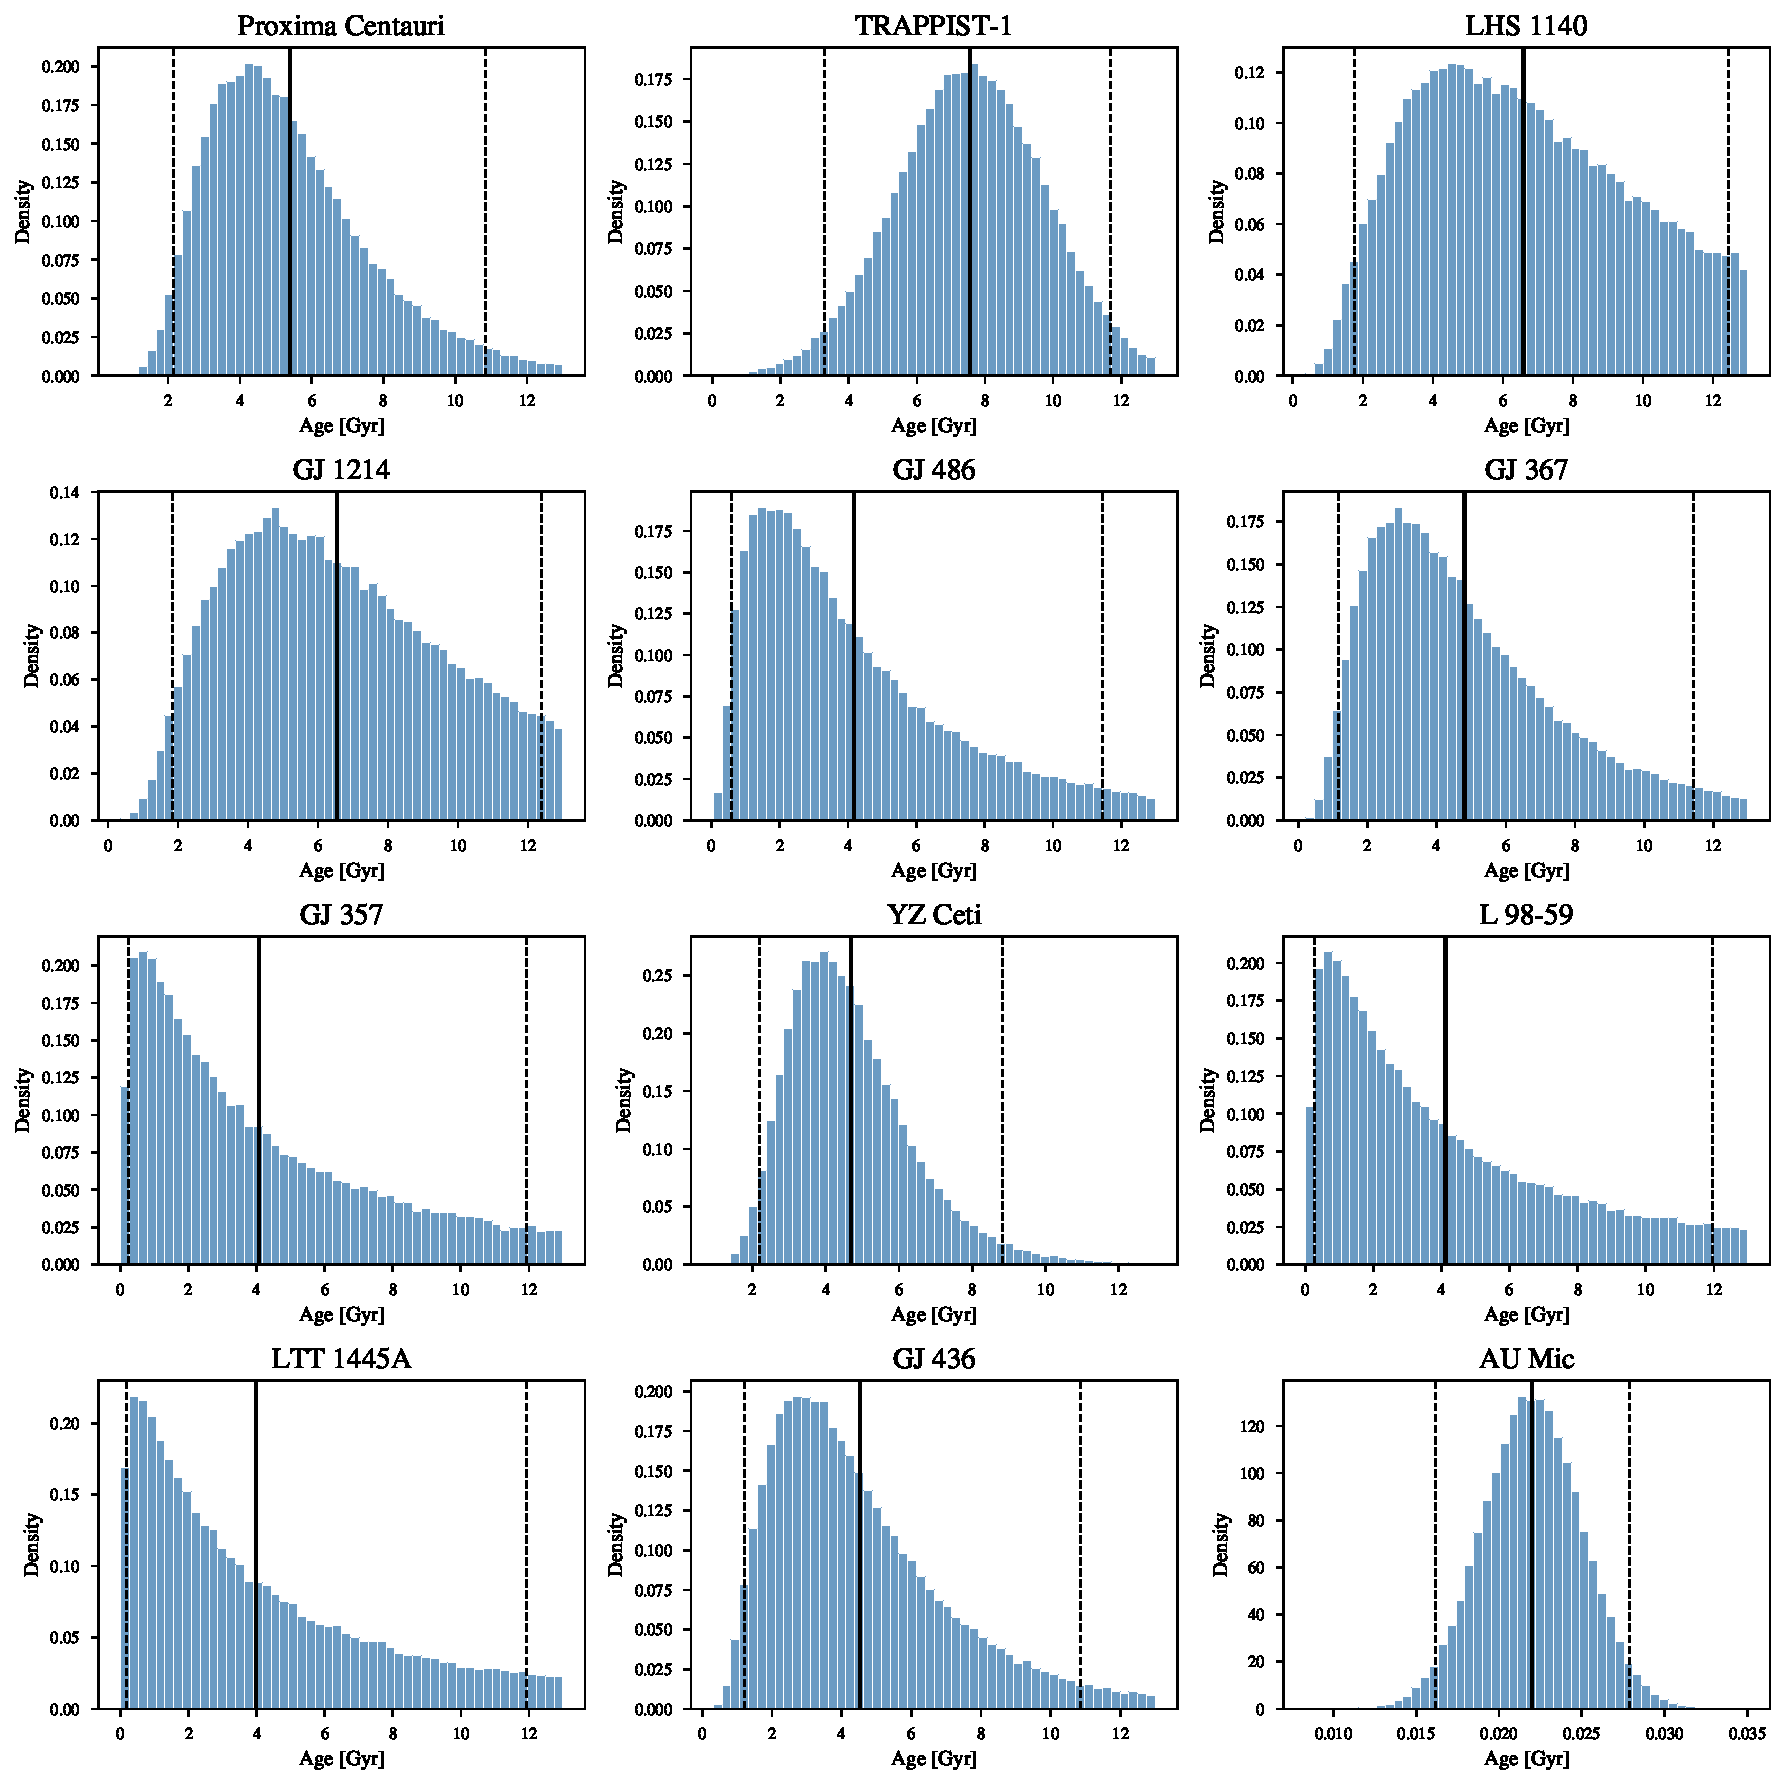
\includegraphics[width=\columnwidth]{age_distributions.pdf}
  \caption{Posterior age distributions for the 12 M~dwarf systems in our
    sample, derived from Monte Carlo sampling of the
    \citet{EngleGuinan2023} rotation-age model. Vertical dashed lines
    indicate the median age, and shaded regions denote the 95\% credible
    interval.}
  \label{fig:ages}
\end{figure}

\subsection{Cumulative XUV Flux Distributions} \label{sec:results_flux}

Table~\ref{tab:fluxes} presents the planetary properties and cumulative XUV
flux estimates for all 25 planets in the sample. Cumulative XUV fluxes
are normalized to $\Fearth$.

\begin{deluxetable*}{lcccccccc}
\tablecaption{Planet Properties and Cumulative XUV Fluxes\label{tab:fluxes}}
\tablehead{
\colhead{Planet} & \colhead{$P_{\rm orb}$ [d]} & \colhead{$M_p$ [$M_\oplus$]} & \colhead{$v_{\rm esc}$ [km/s]} & \colhead{$F_{\rm XUV}/F_\oplus$} & \colhead{$F_{\rm shore}/F_\oplus$} & \colhead{$\Delta_{\rm shore}$} & \colhead{95\% CI} & \colhead{Atmosphere}
}
\startdata
Proxima Centauri b & 11.1868 & 1.07 & 11.5 & $15.9_{-5.1}^{+6.1}$ & 1.1 & 14.40 & [10.8, 22.0] & Vulnerable \\
TRAPPIST-1 b & 1.5109 & 1.37 & 12.6 & $176.5_{-48.6}^{+59.1}$ & 1.6 & 110.50 & [127.9, 235.6] & Vulnerable \\
TRAPPIST-1 c & 2.4218 & 1.31 & 12.3 & $94.1_{-25.9}^{+31.5}$ & 1.5 & 63.33 & [68.2, 125.6] & Vulnerable \\
TRAPPIST-1 d & 4.0496 & 0.39 & 7.9 & $47.4_{-13.0}^{+15.9}$ & 0.2 & 191.25 & [34.3, 63.3] & Vulnerable \\
TRAPPIST-1 e & 6.0996 & 0.69 & 9.8 & $27.4_{-7.6}^{+9.2}$ & 0.6 & 47.23 & [19.9, 36.6] & Vulnerable \\
TRAPPIST-1 f & 9.2067 & 1.04 & 11.3 & $15.9_{-4.4}^{+5.3}$ & 1.1 & 14.99 & [11.5, 21.2] & Vulnerable \\
TRAPPIST-1 g & 12.3529 & 1.32 & 12.4 & $10.7_{-2.9}^{+3.6}$ & 1.5 & 7.11 & [7.8, 14.3] & Vulnerable \\
TRAPPIST-1 h & 18.7674 & 0.33 & 7.4 & $6.1_{-1.7}^{+2.1}$ & 0.2 & 31.99 & [4.4, 8.2] & Vulnerable \\
LHS 1140 c & 3.7779 & 1.81 & 13.9 & $119.3_{-51.1}^{+55.2}$ & 2.4 & 49.76 & [68.1, 174.4] & Vulnerable \\
GJ 1214 b & 1.5804 & 8.17 & 24.1 & $380.5_{-155.8}^{+154.3}$ & 22.1 & 17.23 & [224.7, 534.8] & Vulnerable \\
GJ 486 b & 1.4671 & 3.00 & 16.7 & $704.5_{-480.3}^{+451.8}$ & 5.0 & 139.60 & [224.2, 1156.3] & Vulnerable \\
GJ 367 b & 0.3220 & 0.63 & 9.5 & $5043.7_{-2080.9}^{+2431.0}$ & 0.5 & 9895.03 & [2962.7, 7474.7] & Vulnerable \\
GJ 367 c & 11.5430 & 4.13 & 18.8 & $42.7_{-17.5}^{+20.4}$ & 8.1 & 5.28 & [25.1, 63.1] & Vulnerable \\
GJ 357 b & 3.9306 & 1.84 & 14.0 & $191.7_{-157.3}^{+150.4}$ & 2.5 & 78.05 & [34.4, 342.0] & Vulnerable \\
YZ Ceti b & 2.0208 & 0.70 & 9.8 & $169.9_{-63.2}^{+68.2}$ & 0.6 & 287.38 & [106.7, 238.1] & Vulnerable \\
YZ Ceti c & 3.0601 & 1.14 & 11.7 & $97.7_{-36.3}^{+39.2}$ & 1.2 & 80.54 & [61.4, 136.9] & Vulnerable \\
YZ Ceti d & 4.6564 & 1.09 & 11.5 & $55.8_{-20.7}^{+22.4}$ & 1.1 & 49.16 & [35.1, 78.3] & Vulnerable \\
L 98-59 b & 2.2531 & 0.40 & 8.0 & $301.3_{-241.3}^{+278.2}$ & 0.3 & 1162.34 & [59.9, 579.4] & Vulnerable \\
L 98-59 c & 3.6906 & 2.22 & 15.0 & $156.0_{-125.0}^{+144.1}$ & 3.2 & 48.18 & [31.0, 300.1] & Vulnerable \\
L 98-59 d & 7.4507 & 1.94 & 14.2 & $61.1_{-49.0}^{+56.5}$ & 2.7 & 23.03 & [12.1, 117.6] & Vulnerable \\
LTT 1445A b & 5.3588 & 2.87 & 16.4 & $84.9_{-70.2}^{+72.8}$ & 4.7 & 17.97 & [14.8, 157.7] & Vulnerable \\
LTT 1445A c & 3.1239 & 1.54 & 13.1 & $174.4_{-144.2}^{+149.5}$ & 1.9 & 92.33 & [30.3, 323.9] & Vulnerable \\
GJ 436 b & 2.6439 & 21.36 & 34.2 & $298.1_{-120.7}^{+166.4}$ & 91.0 & 3.28 & [177.4, 464.6] & Vulnerable \\
AU Mic b & 8.4630 & 17.10 & 31.5 & $13.7_{-7.6}^{+13.7}$ & 65.6 & 0.21 & [6.1, 27.4] & Protected \\
AU Mic c & 18.8590 & 9.60 & 25.5 & $4.7_{-2.6}^{+4.7}$ & 28.0 & 0.17 & [2.1, 9.4] & Protected \\
\enddata
\tablecomments{Cumulative XUV fluxes normalized to Earth's value ($F_\oplus = 9.76 \times 10^{15}$ W/m$^2$). $F_{\rm shore}$ is the cosmic shoreline flux (Zahnle \& Catling 2017). $\Delta_{\rm shore} = F_{\rm XUV}/F_{\rm shore}$; values $> 1$ indicate the planet lies on the atmosphere-vulnerable side of the shoreline.}
\end{deluxetable*}

Figure~\ref{fig:flux} shows the cumulative XUV flux distributions for all
planets.

\begin{figure}[ht!]
  \centering
  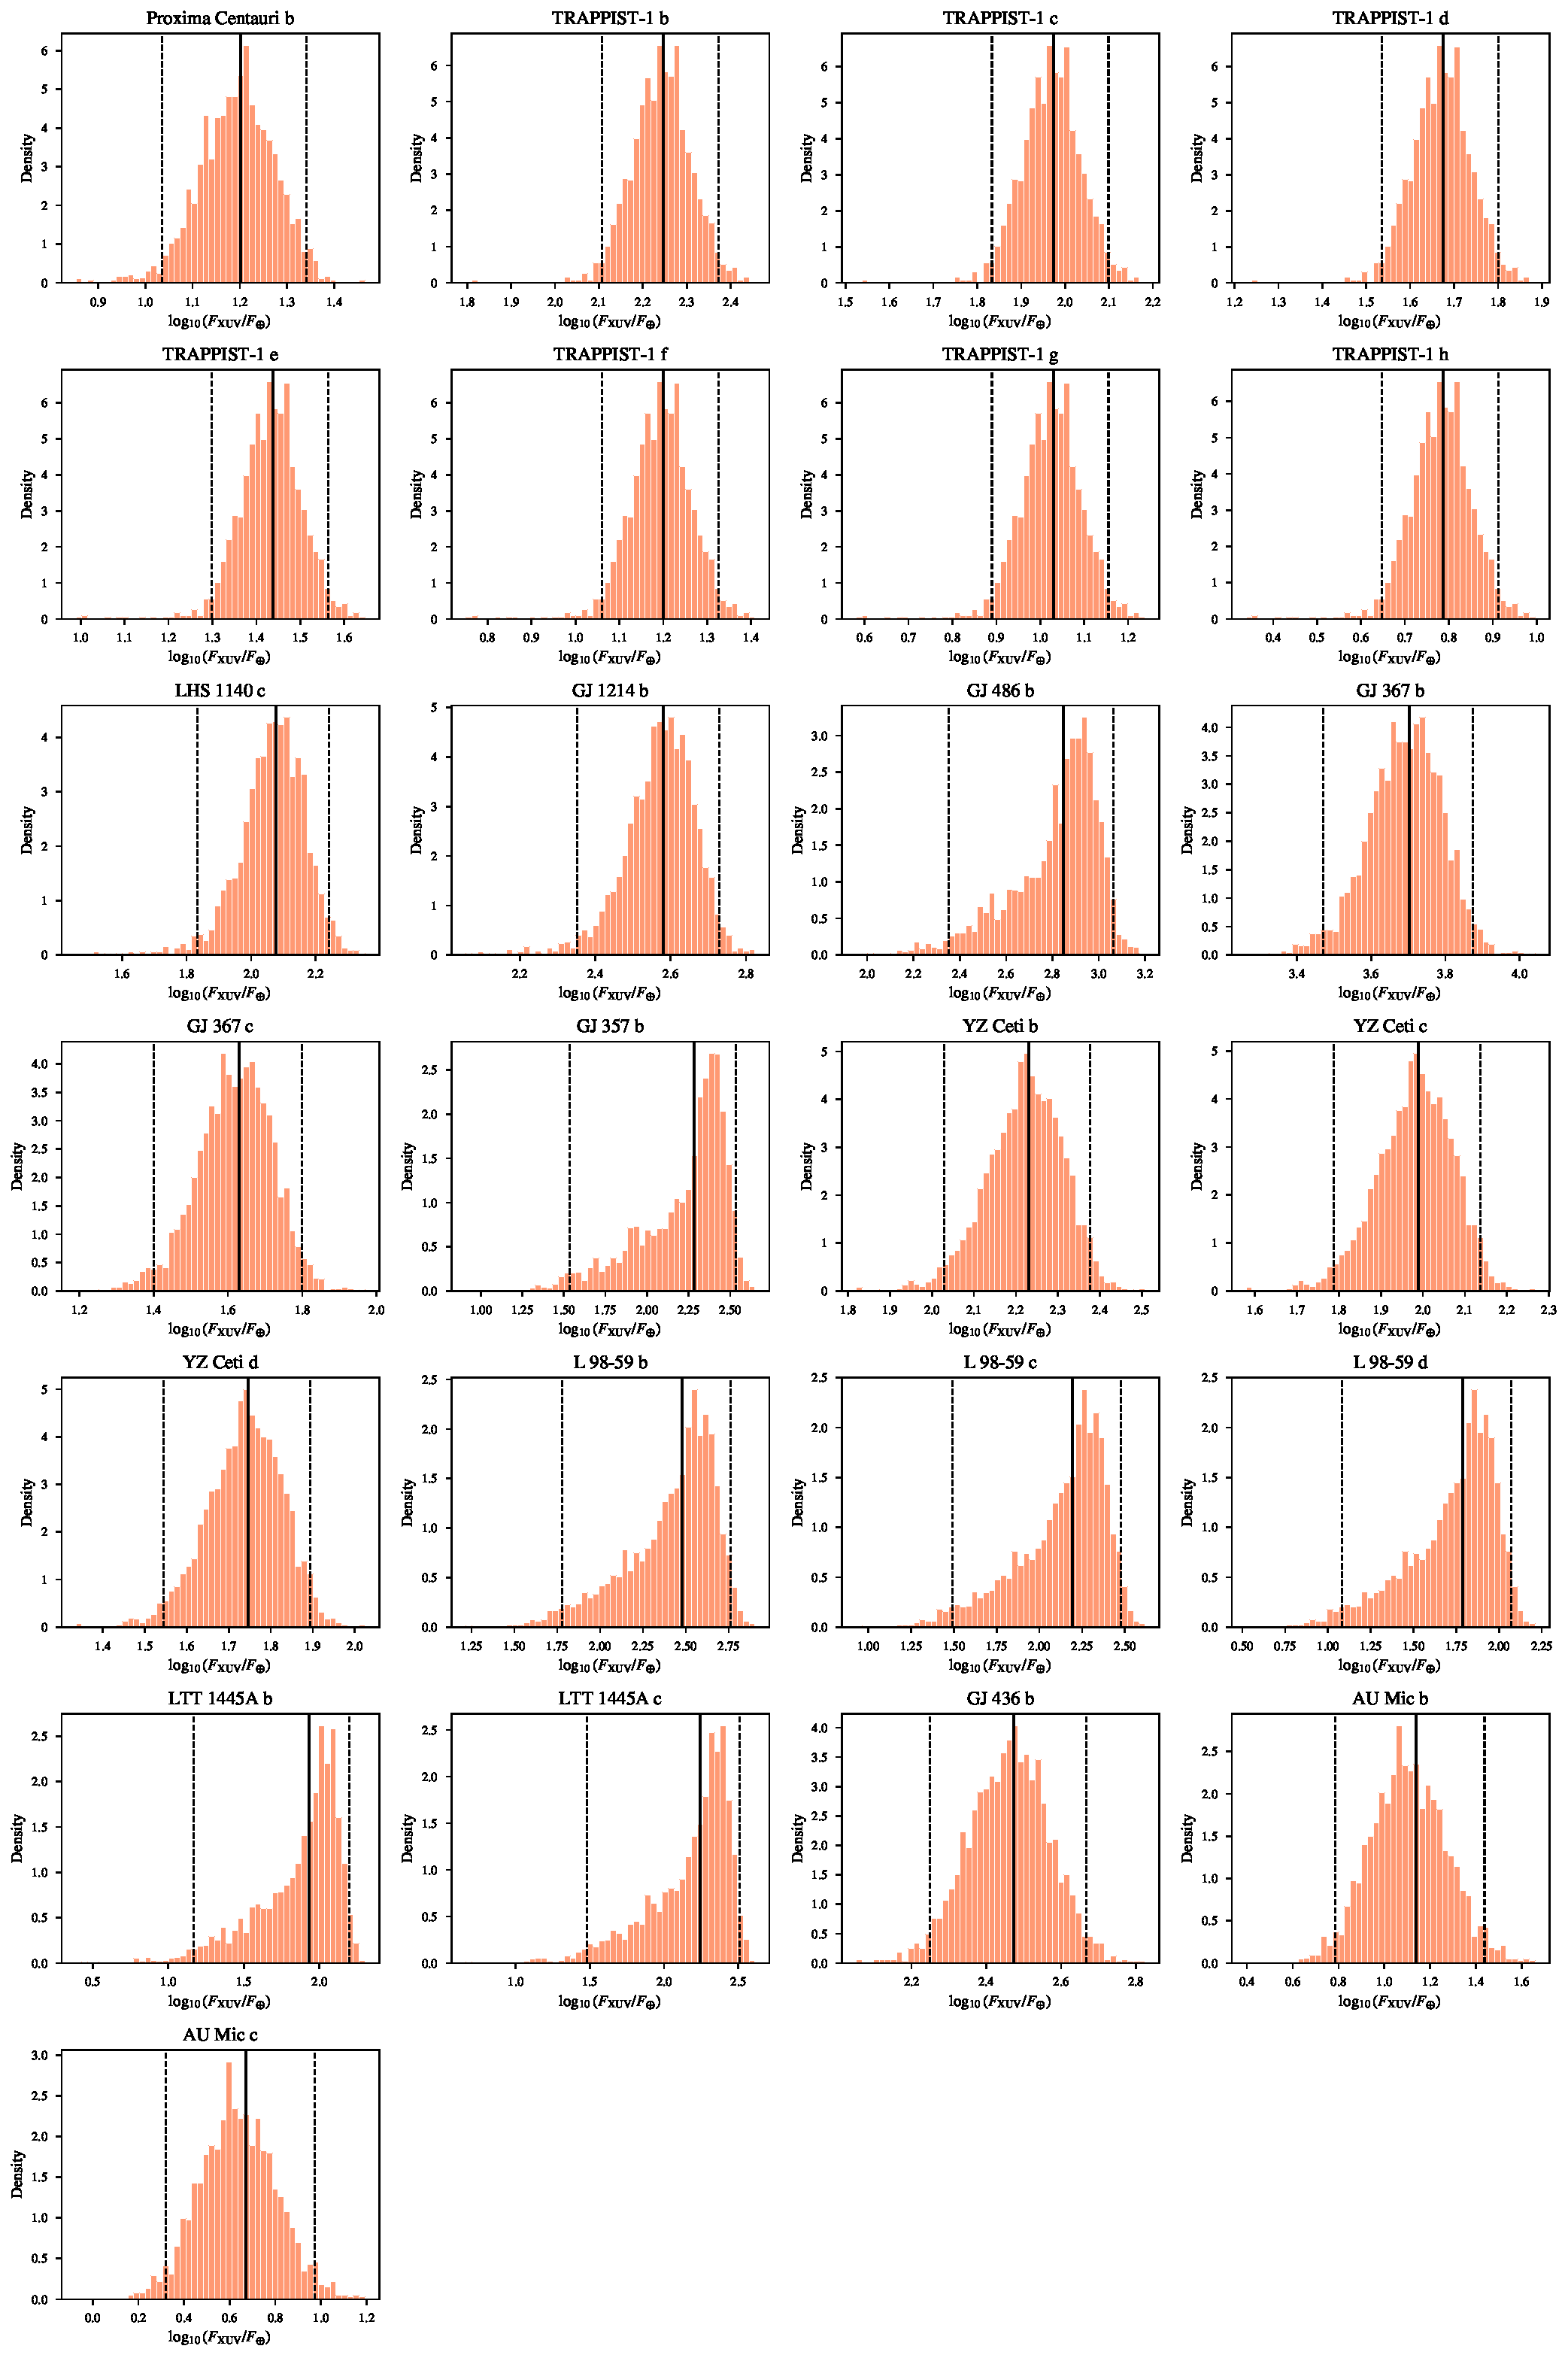
\includegraphics[width=\columnwidth]{flux_distributions.pdf}
  \caption{Posterior distributions of the cumulative XUV flux normalized to
    the Earth value ($\Fcum / \Fearth$) for all planets in the sample.
    Vertical dashed lines indicate the median, and shaded regions denote the
    95\% credible interval.}
  \label{fig:flux}
\end{figure}

\subsection{Cosmic Shoreline} \label{sec:results_shoreline}

Figure~\ref{fig:shoreline} places all planets on the cosmic shoreline diagram
of \citet{ZahnleCatling2017}, plotting escape velocity against normalized
cumulative XUV flux.

\begin{figure*}[ht!]
  \centering
  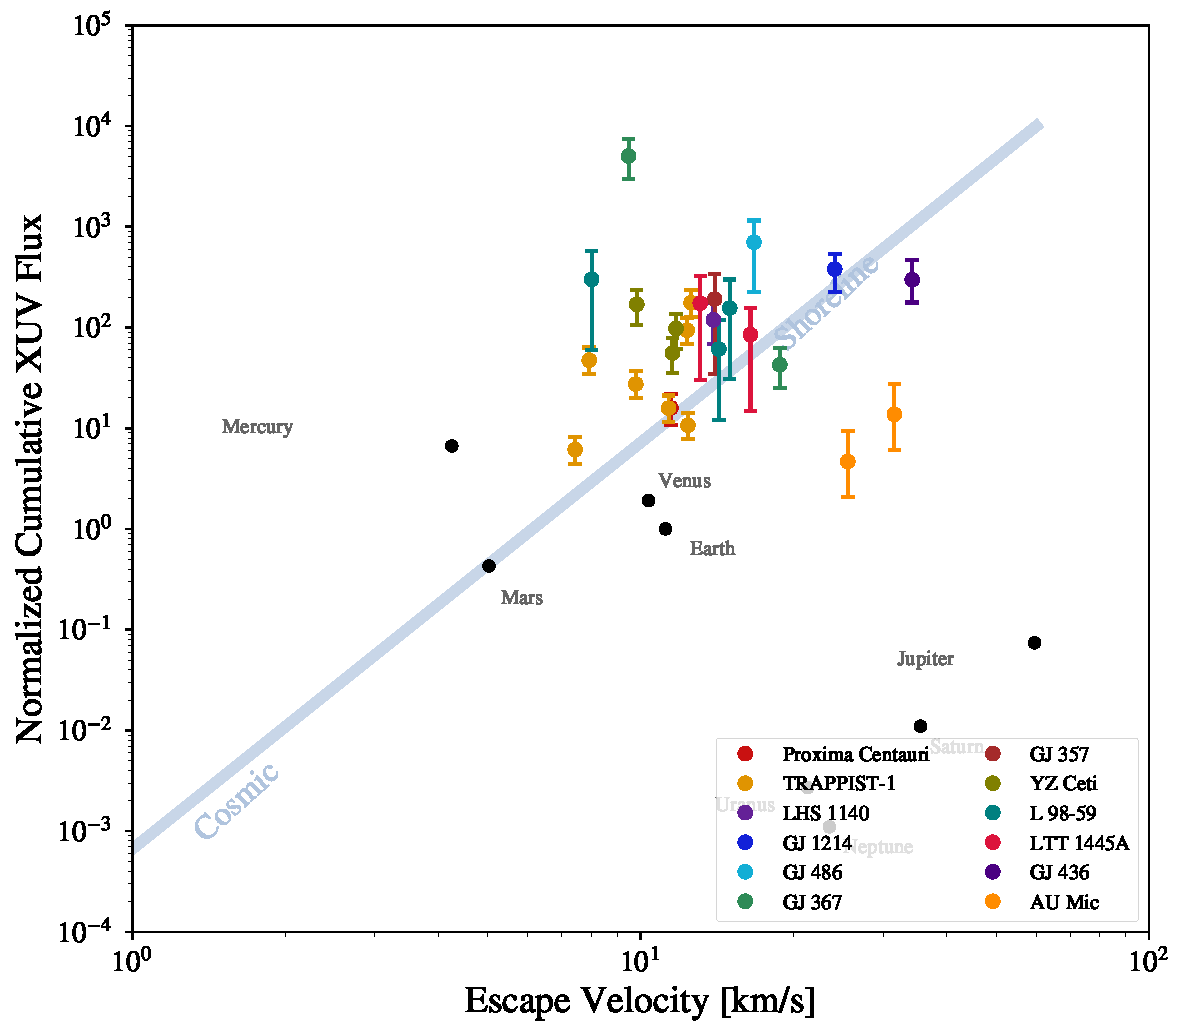
\includegraphics[width=\textwidth]{cosmic_shoreline.pdf}
  \caption{Cosmic shoreline diagram after \citet{ZahnleCatling2017}. Each
    planet is plotted with its escape velocity on the horizontal axis and the
    median normalized cumulative XUV flux on the vertical axis. Error bars
    denote the 95\% credible interval of $\Fcum / \Fearth$. The diagonal band
    indicates the empirical cosmic shoreline. Solar System planets are shown as
    black circles for reference. Nearly all M~dwarf planets in our sample lie
    above the shoreline, on the atmosphere-vulnerable side; the exceptions are
    AU~Mic~b and c, which lie below due to the system's extreme youth.}
  \label{fig:shoreline}
\end{figure*}

\clearpage
%% ============================================================================
\section{Discussion} \label{sec:discussion}

\subsection{Atmospheric Vulnerability Across the Sample}

Nearly all planets in our sample lie above the cosmic shoreline of
\citet{ZahnleCatling2017}, indicating that their cumulative XUV exposures
exceed the empirical threshold for atmospheric retention given their escape
velocities. This result is expected for close-in planets around M~dwarfs, which
experience both intense XUV irradiation and prolonged pre-main-sequence
saturation phases.

The most extreme case is GJ~367~b, an ultra-short-period planet ($P = 0.32$~d)
with a cumulative XUV flux $\sim$5000 times Earth's value, placing it firmly in
the atmosphere-stripped regime consistent with its classification as a dense,
Mercury-like body \citep{Goffo2023}. In contrast, the outer TRAPPIST-1 planets
(f, g, h) receive cumulative XUV fluxes only $\sim$6--16 times Earth's value,
suggesting comparatively modest atmospheric erosion despite their proximity to
the cosmic shoreline.

The two AU~Mic planets are the only objects in our sample that lie below the
cosmic shoreline, with cumulative XUV fluxes of $\sim$14$\,\Fearth$ (b) and
$\sim$5$\,\Fearth$ (c). This is a direct consequence of the system's extreme
youth ($\sim$20~Myr): despite intense instantaneous XUV irradiation, the
planets have simply not had sufficient time to accumulate large cumulative
exposures. Their high masses ($17.1$ and $9.6\,\Mearth$) also place them at
high escape velocities, raising the shoreline threshold. As AU~Mic ages, these
planets will cross the shoreline and enter the atmosphere-vulnerable regime.

\subsection{The TRAPPIST-1 System}

The seven TRAPPIST-1 planets span a factor of $\sim$30 in cumulative XUV flux,
from 176$\,\Fearth$ for planet~b to 6$\,\Fearth$ for planet~h. This gradient
provides a natural laboratory for studying atmospheric retention as a function
of XUV exposure. Planets f and g, which receive cumulative XUV fluxes
comparable to Proxima Centauri~b ($\sim$16$\,\Fearth$), are among the least
irradiated in the sample and may represent the most favorable targets for
atmospheric characterization.

We note that TRAPPIST-1's stellar mass ($0.0898\,\Msun$) falls below the
calibration range of the \citet{Engle2024} mid-to-late M~dwarf XUV model,
which requires $M_\star > 0.10\,\Msun$. We adopted the minimum valid mass
($0.101\,\Msun$) for the XUV evolution calculation. This approximation
introduces a systematic uncertainty that slightly overestimates the XUV
luminosity, making our cumulative flux estimates for the TRAPPIST-1 planets
conservative upper bounds.

\subsection{Comparison of XUV Flux Uncertainty Widths}

The width of the cumulative XUV flux posterior varies substantially across our
sample. GJ~486~b and GJ~357~b show the broadest distributions (spanning nearly
an order of magnitude in their 95\% credible intervals), reflecting large
uncertainties in their stellar rotation periods and consequently their ages.
In contrast, the TRAPPIST-1 planets show narrow distributions (factor of
$\sim$2), benefiting from the independent age constraint of
\citet{BurgasserMamajek2017}. This comparison underscores the importance of
precise rotation period measurements and independent age indicators for
constraining cumulative XUV histories.

\subsection{Caveats}

Several simplifications in our analysis warrant discussion. First, we use the
mass-radius relation $R \propto M^{0.27}$ to estimate planetary radii and
escape velocities, which may not apply to all planets in the sample (e.g.,
the sub-Neptune GJ~1214~b). Second, the \citet{Engle2024} XUV model is
calibrated on a limited sample of benchmark stars, and systematic uncertainties
in the calibration are not propagated into our results. Third, we do not model
atmospheric escape self-consistently; our cumulative XUV fluxes represent the
total energy incident on the planet, not the actual mass lost.

%% ============================================================================
\section{Conclusions} \label{sec:conclusions}

We have computed cumulative XUV flux probability distributions for 25
planets with orbital periods $P < 25$~days around 12 nearby M~dwarf systems.
Our main findings are:

\begin{enumerate}
  \item Nearly all planets in the sample lie above the cosmic shoreline of
    \citet{ZahnleCatling2017}, receiving cumulative XUV fluxes 5--5000 times
    Earth's value. The exceptions are AU~Mic~b and c, whose extreme youth
    ($\sim$20~Myr) has limited their cumulative exposures.
  \item The TRAPPIST-1 system spans a factor of $\sim$30 in cumulative XUV
    flux, with the outer planets (f, g, h) receiving the lowest exposures
    among the mature systems ($\sim$6--16$\,\Fearth$).
  \item The width of the cumulative XUV flux posterior depends strongly on the
    precision of the stellar age estimate, highlighting the value of
    independent age constraints.
  \item Ultra-short-period planets such as GJ~367~b receive extreme cumulative
    XUV exposures ($\sim$5000$\,\Fearth$), consistent with complete atmospheric
    stripping.
\end{enumerate}

These distributions provide a quantitative basis for prioritizing atmospheric
characterization targets with JWST and future observatories. Planets with lower
cumulative XUV exposures relative to their escape velocities---such as
TRAPPIST-1~f and~g, and GJ~1214~b---are the most promising candidates for
retaining detectable atmospheres.

\begin{acknowledgments}
This research made use of \vplanet{} \citep{Barnes2020}, \vconverge{}, and
the NASA Exoplanet Archive.
\end{acknowledgments}

\bibliography{references}

\end{document}
